\documentclass[11pt,reqno]{amsart}
\usepackage[top=1in, left=1in, right=1in, bottom=1in]{geometry}                % See geometry.pdf to learn the layout options. There are lots.
\geometry{letterpaper}                   % ... or a4paper or a5paper or ...
\usepackage[parfill]{parskip}    % Activate to begin paragraphs with an empty line rather than an indent
%\usepackage{algorithm, algorithmic}

\usepackage{algorithm}
\usepackage{algpseudocode}
\usepackage{hyperref}
\usepackage{graphicx}
%\usepackage{url}
%\usepackage{verbatim}
\usepackage{amssymb}
\usepackage{amsmath}
\usepackage{enumitem}
\usepackage{setspace}
\doublespacing
\usepackage{natbib}


\newcommand{\RR}{I\!\!R} %real numbers
\DeclareMathOperator{\diag}{diag}

\algnewcommand{\Inputs}[1]{%
  \State \textbf{Inputs:}
  \Statex \hspace*{\algorithmicindent}\parbox[t]{.8\linewidth}{\raggedright #1}
}
\algnewcommand{\Initialize}[1]{%
  \State \textbf{Initialize:}
  \Statex \hspace*{\algorithmicindent}\parbox[t]{.8\linewidth}{\raggedright #1}
}

\title[]{Review on Rare Variants Detection Methods}
\author{Fan Zhang}                                          

\begin{document}
\maketitle

\section{Why do we need a sensitive variant detection method?}
\subsection{Errors in NGS data}
\subsection{Variants}
\subsubsection{Germline, somatic, or LOH (loss of heterozygosity)}
\subsubsection{Rare and common variants}

\section{Hallmarks of a good variant detection method}
\subsection{Accuracy}
\subsection{Scalability}
\subsection{Robustness}

\section{Factors that effect the ability of variant detection methods}
coverage of NGS data, allele fraction...

\section{Criteria for choosing a variant detection method}
It depends on specific purposes.

\section{Classification for variant detection methods}
We classify the state-of-the-art variant detection methods into two categories - probabilistic methods and non-probabilistic methods (Table~\ref{tbl:methods}).
\begin{table}[!ht]
\centering
%\vspace{10pt}
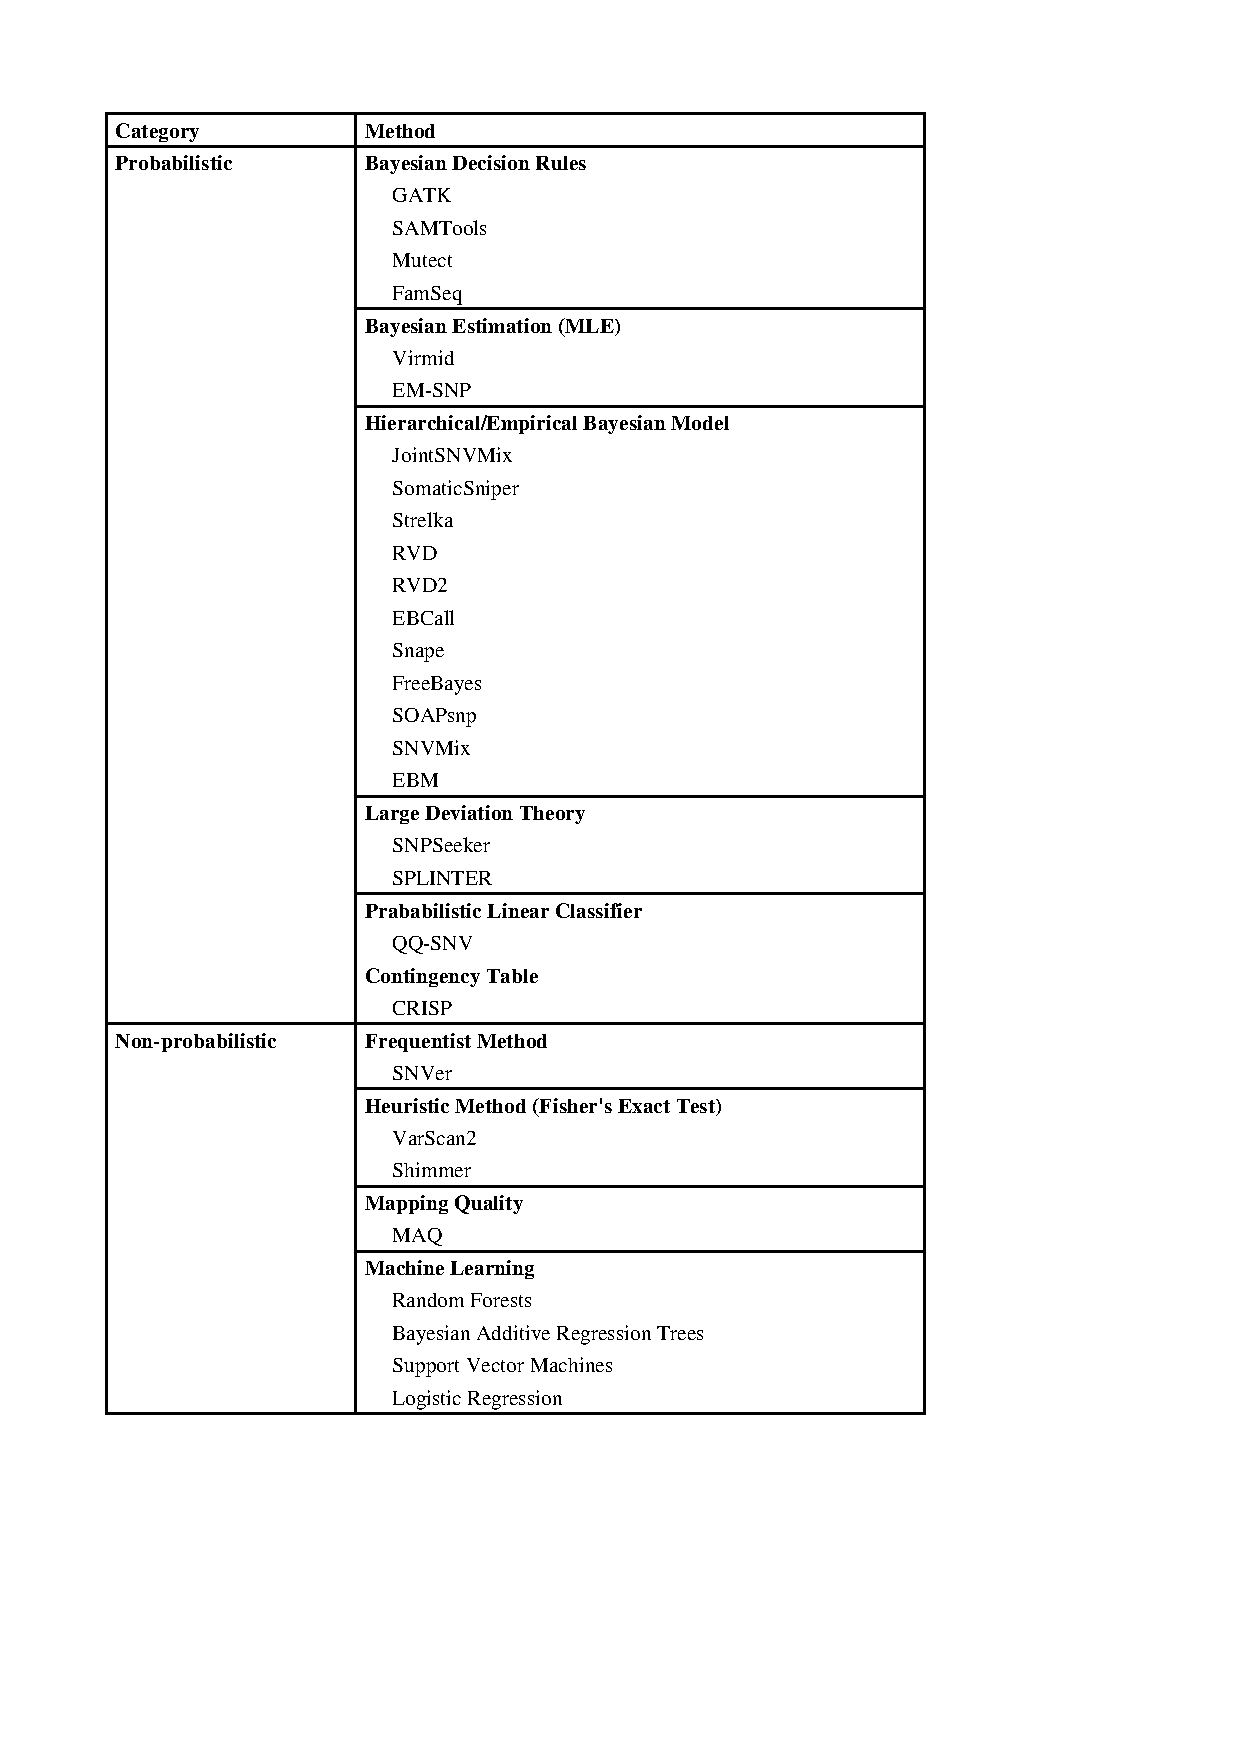
\includegraphics[width=1.1\textwidth]{method_table.pdf}
\caption{Single nucleotide variant detection methods.}
%\vspace{-10p}
\label{tbl:methods}
\end{table}


\subsection{Probabilistic Methods}
List of 21 probabilistic methods for variant detection:

GATK \citep{McKenna2010},

SAMTools \citep{Li2009a},

Mutect \citep{Cibulskis2013},

FamSeq \citep{Peng2013},

Virmid \citep{Kim2013},

EM-SNP \citep{Chen2013},

JointSNVMix \citep{Roth2012},

SomaticSniper \citep{Larson2012},

Strelka \citep{Saunders2012},

RVD \citep{Flaherty2012},

RVD2 \citep{He2015},

EBCall \citep{Shiraishi2013},

Snape \citep{Raineri2012},

FreeBayes \citep{Garrison2012},

SOAPsnp \citep{Li2009},

SNVMix \citep{Goya2010},

EBM \citep{Zhou2012},

SNPSeeker \citep{Druley2009},

SPLINTER \citep{Spencer2014},

QQ-SNV \citep{VanderBorght2015},

CRISP \citep{Bansal2010}.

\subsection{Non-probabilistic Methods}
List of 8 non-probabilistic methods for variant detection:

SNVer \citep{Wei2011},

VarScan2 \citep{Koboldt2012},

Shimmer \citep{Hansen2013},

MAQ \citep{Li2008},

Random Forests \citep{Ding2012},

Bayesian Additive Regression Trees \citep{Ding2012},

Support Vector Machines \citep{Ding2012},

Logistic Regression \citep{Ding2012}.


\bibliographystyle{apalike}
\bibliography{bib}
\end{document}
